\documentclass[12pt,a4paper]{article}
\usepackage[utf8]{inputenc}
\usepackage[english]{babel}

\usepackage{amsmath}
\usepackage{amsfonts}
\usepackage{amssymb}

\usepackage{graphicx}
\usepackage{caption}
\usepackage{subcaption}
\usepackage{lmodern}
\usepackage{tikz}
\usetikzlibrary{calc}
\usepackage{titlesec}
\usepackage{environ}
\usepackage{xcolor}
\usepackage{fancyhdr}
\usepackage[colorlinks = true, linkcolor = black]{hyperref}
\usepackage{xparse}
\usepackage{enumitem}
\usepackage{comment}
\usepackage{wrapfig}
\usepackage[capitalise]{cleveref}

\usepackage[left=2cm,right=2cm,top=2cm,bottom=2cm]{geometry}
\usepackage{multicol}
\usepackage[indent=0pt]{parskip}

\newcommand{\spaceP}{\vspace*{0.5cm}}
\newcommand{\Span}{\mathrm{Span}\,}
\newcommand{\range}{\mathrm{range}\,}
\newcommand{\ra}{\rightarrow}

%% Redefining sections
\newcommand{\sectionformat}[1]{%
    \begin{tikzpicture}[baseline=(title.base)]
        \node[rectangle, draw] (title) {#1};
    \end{tikzpicture}
    
    \noindent\hrulefill
}

\newif\ifhNotes 

\hNotesfalse

\ifhNotes
	\newcommand{\hideNotes}[1]{%
	\phantom{#1}
	}
	\newcommand{\hideNotesU}[1]{%
	\underline{\hspace{1mm}\phantom{#1}\hspace{1mm}}
	}
\else
	\newcommand{\hideNotes}[1]{#1}
	\newcommand{\hideNotesU}[1]{\textcolor{blue}{#1}}
\fi

% default values copied from titlesec documentation page 23
% parameters of \titleformat command are explained on page 4
\titleformat%
    {\section}% <command> is the sectioning command to be redefined, i. e., \part, \chapter, \section, \subsection, \subsubsection, \paragraph or \subparagraph.
    {\normalfont\large\scshape}% <format>
    {}% <label> the number
    {0em}% <sep> length. horizontal separation between label and title body
    {\centering\sectionformat}% code preceding the title body  (title body is taken as argument)

%% Set counters for sections to none
\setcounter{secnumdepth}{0}

%% Set the footer/headers
\pagestyle{fancy}
\fancyhf{}
\renewcommand{\headrulewidth}{0pt}
\renewcommand{\footrulewidth}{2pt}
\lfoot{P.-O. Paris{\'e}}
\cfoot{MATH 241}
\rfoot{Page \thepage}

%% Defining example environment
\newcounter{example}[section]
\NewEnviron{example}%
	{%
	\noindent\refstepcounter{example}\fcolorbox{gray!40}{gray!40}{\textsc{\textcolor{red}{Example~\theexample.}}}%
	%\fcolorbox{black}{white}%
		{  %\parbox{0.95\textwidth}%
			{
			\BODY
			}%
		}%
	}

% Theorem environment
\NewEnviron{theorem}%
	{%
	\noindent\refstepcounter{example}\fcolorbox{gray!40}{gray!40}{\textsc{\textcolor{blue}{Theorem~\theexample.}}}%
	%\fcolorbox{black}{white}%
		{  %\parbox{0.95\textwidth}%
			{
			\BODY
			}%
		}%
	}

\NewEnviron{notes}%
	{%
	\noindent \fcolorbox{gray!40}{gray!40}{\textsc{\textcolor{blue}{Solution.}}}%
	%\fcolorbox{black}{white}%
		{  %\parbox{0.95\textwidth}%
			{
			\textcolor{blue}{%
			\BODY
			}
			}%
		}%
	}
%%% Ignorer les notes
\excludecomment{notes}

%%%%
\begin{document}
\thispagestyle{empty}

\begin{center}
\vspace*{2.5cm}

{\Huge \textsc{Math 241}}

\vspace*{2cm}

{\LARGE \textsc{Chapter 4}} 

\vspace*{0.75cm}

\noindent\textsc{Section 4.1: Areas and Distances}

\vspace*{0.75cm}

\tableofcontents

\vfill

\noindent \textsc{Created by: Pierre-Olivier Paris{\'e}} \\
\textsc{Fall 2022}
\end{center}

\newpage

\section{Area Problem}

	What is the area of the following shapes?
	
	\begin{figure}[ht]
		\centering
		\begin{subfigure}[b]{0.32\textwidth}
			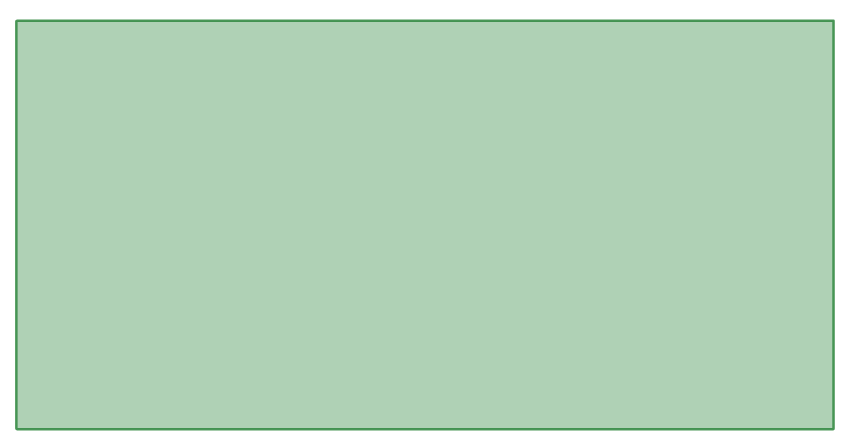
\includegraphics[scale=0.18]{rectangle.png}
			\caption{$\text{Area} = $ \phantom{AAAAA}}
		\end{subfigure}
		\hfill
		\begin{subfigure}[b]{0.32\textwidth}
			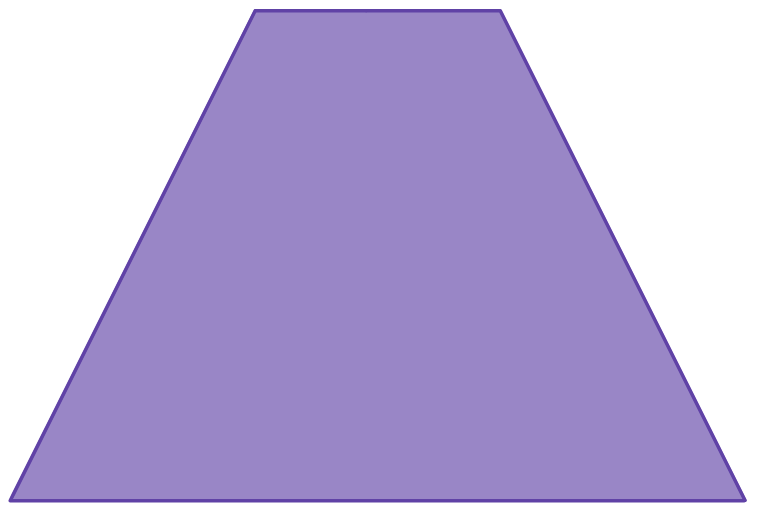
\includegraphics[scale=0.18]{trapezoide.png}
			\caption{$\text{Area} = $ \phantom{AAAAA}}
		\end{subfigure}
		\hfill
		\begin{subfigure}[b]{0.32\textwidth}
			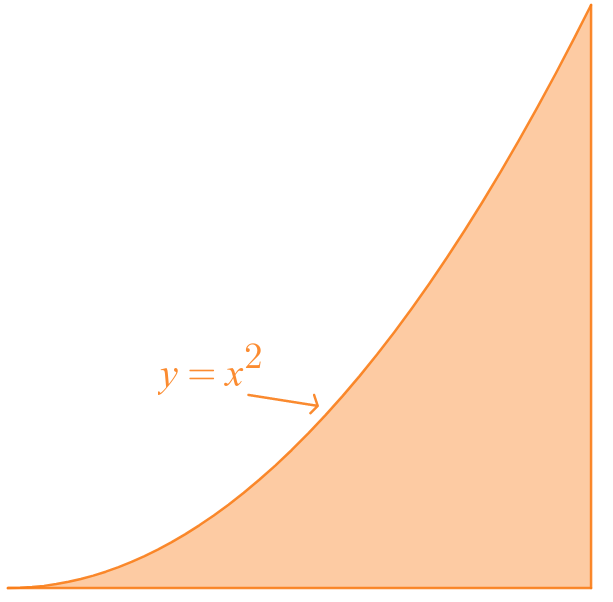
\includegraphics[scale=0.25]{parabola.png}
			\caption{$\text{Area} = $ \phantom{AAAAA}}
		\end{subfigure}
	\end{figure}
	
	\vspace*{12pt}
	
	\underline{Trick:} Use simpler shapes, such as rectangles, to approximate the area.
	
	\vspace*{12pt}
	
	\begin{example}\label{Ex:ParabolaArea}
	Using rectangles, approximate the area of the region $S$ under the graph of $y= x^2$ between $x = 0$ and $x = 1$. Go to Desmos: \url{https://www.desmos.com/calculator/gfrgqd4nvx}
	\end{example}
	
	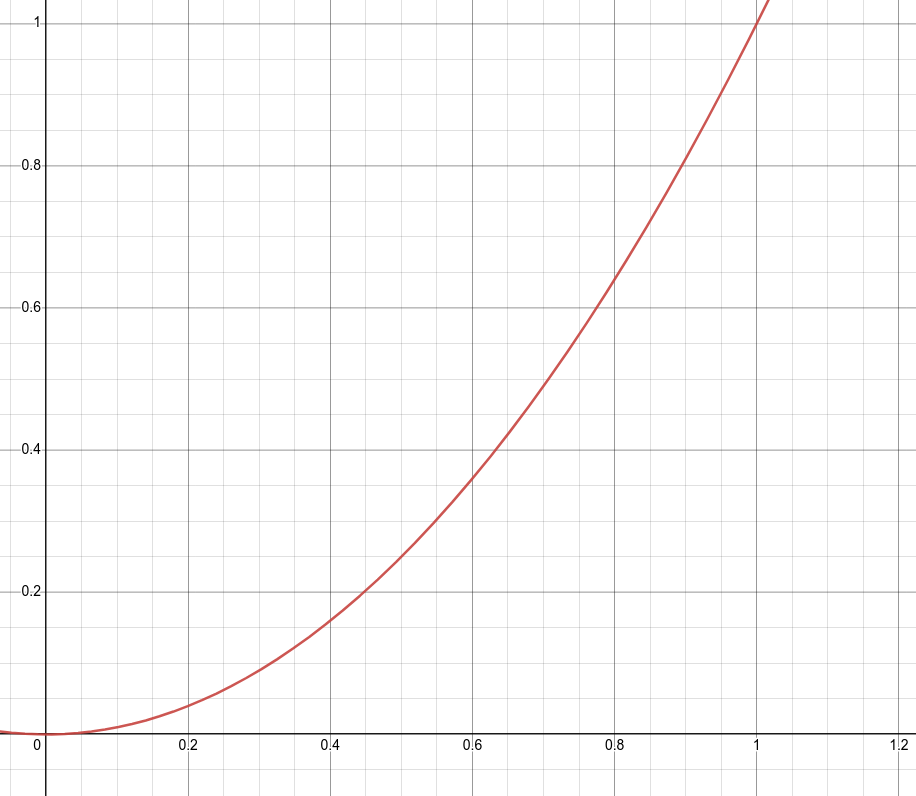
\includegraphics[scale=0.25]{graphOfSquareX.png}
	
	\newpage
	
	\subsection{Divide and Conquer With the Right Endpoint Rule!}
	
	Suppose we want to compute the area of a region $S$ bounded by the graph of some function $y = f(x)$.
	
	\begin{center}
	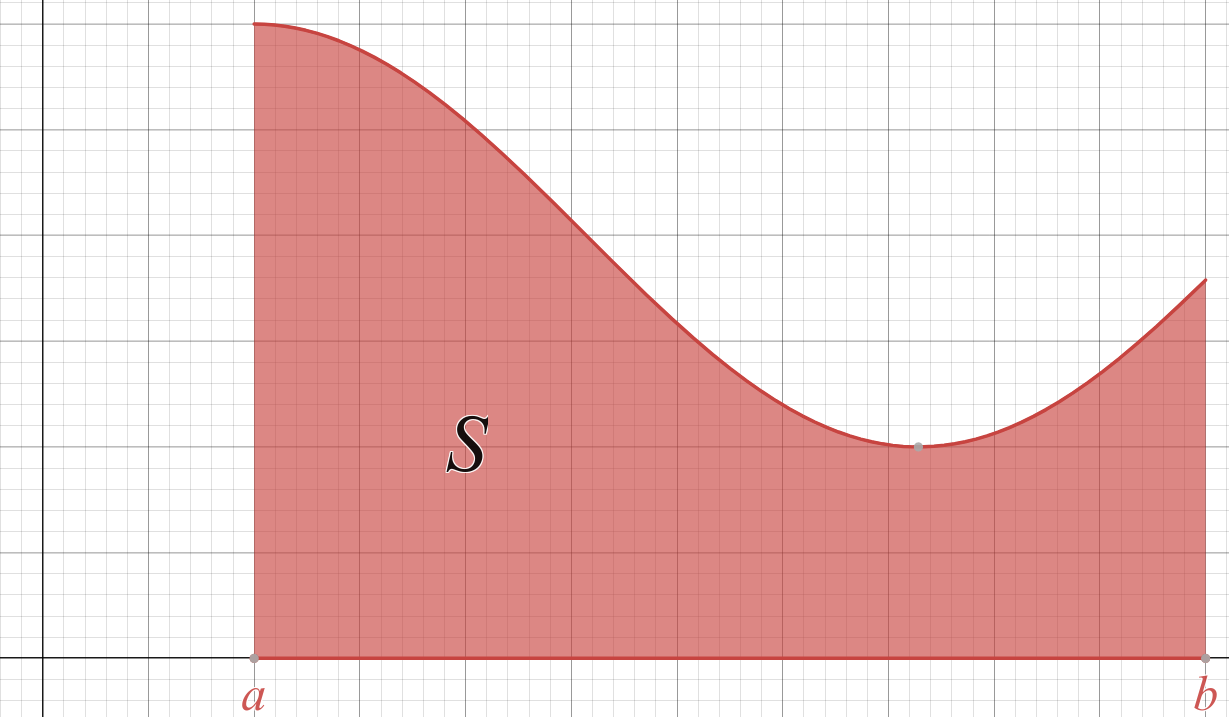
\includegraphics[scale=0.39]{regionS.png}
	\end{center}
	
	\begin{enumerate}[label=\underline{\textsc{Step} \Roman*}]
	\item Subdivide the region $S$ into $n$ strips of equal width $\Delta x = (b-a)/n$.
		\begin{center}
		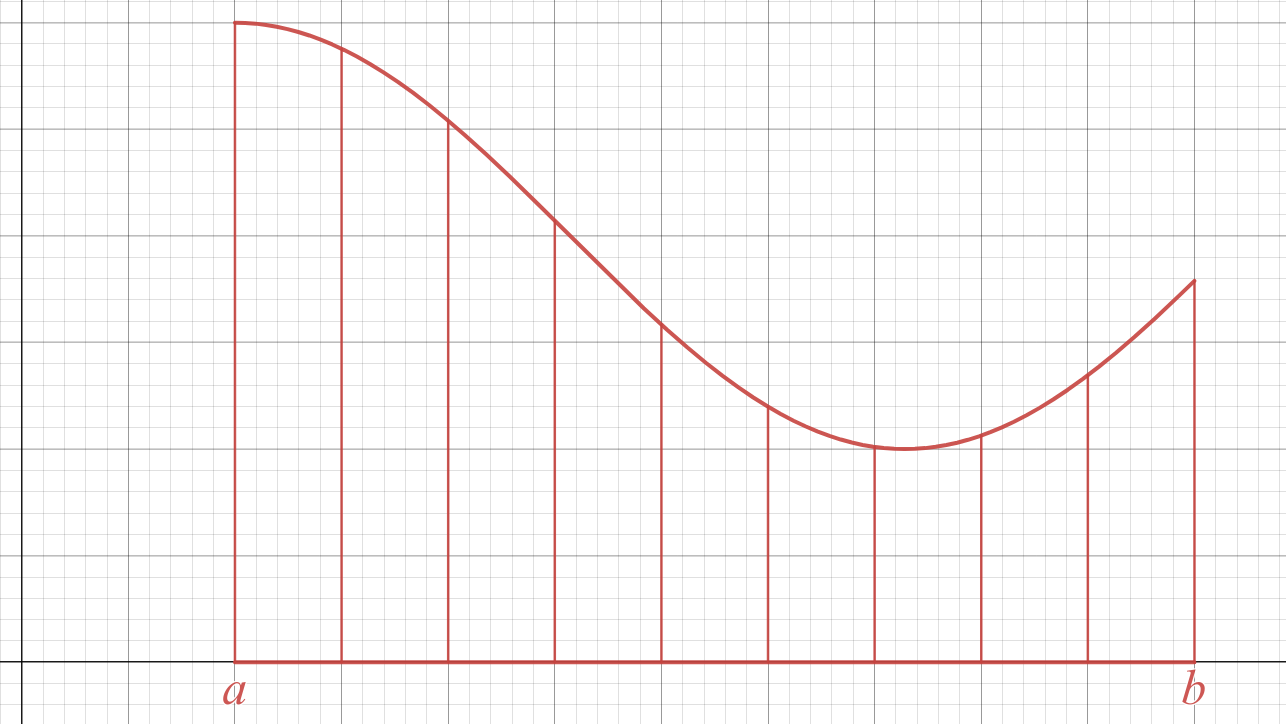
\includegraphics[scale=0.365]{regionSDivided}
		\end{center}
		\vspace*{10pt}
	\item Choose the right-end point for all subintervals:\\
		$x_1 = a + \Delta x$, $x_2 = a + 2 \Delta x$, $\ldots$, $x_{n-1} = a + (n - 1) \Delta x$, $x_n = b$.
	\item Approximate by adding the area of each rectangle:
		\begin{align*}
		R_n = f(x_1) \Delta x + f(x_2) \Delta x + \cdots + f(x_n) \Delta x .
		\end{align*}
	\end{enumerate}
	
	\newpage
	
	\subsection{Divide and Conquer With the Left Endpoint Rule!}
	
	Suppose we want to compute the area of a region $S$ bounded by the graph of some function $y = f(x)$ from $x = a$ to $x = b$.
	
	\begin{center}
	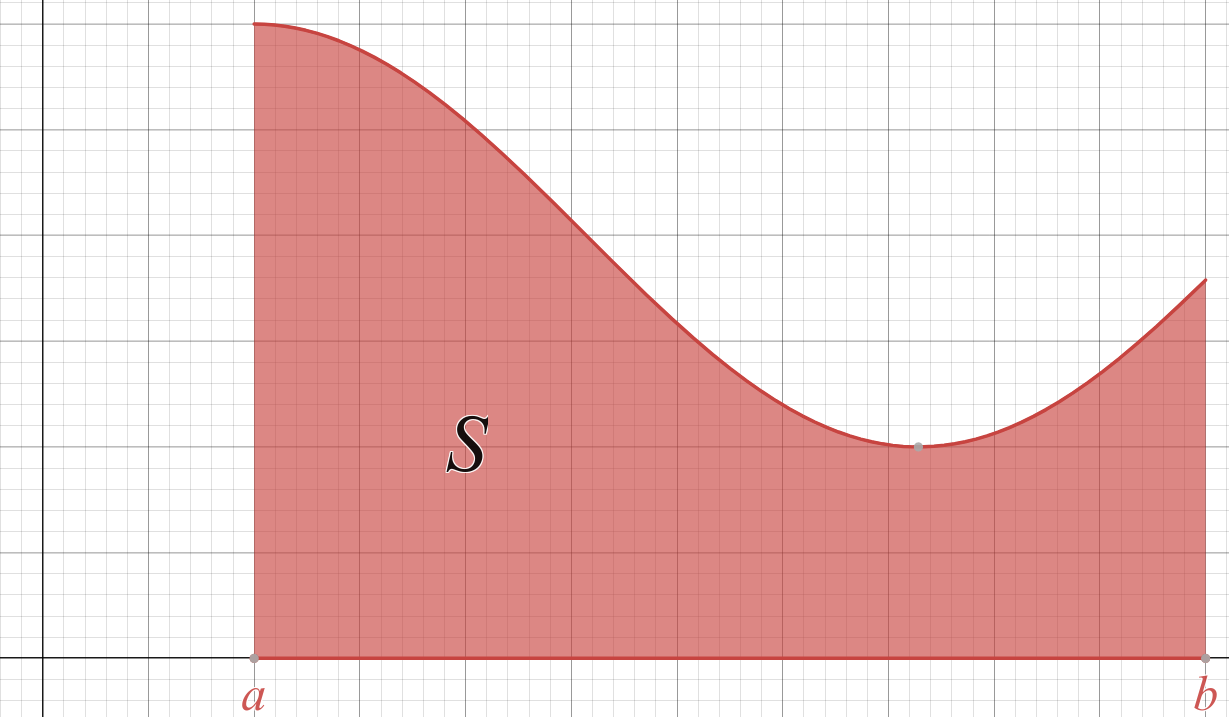
\includegraphics[scale=0.39]{regionS.png}
	\end{center}
	
	\begin{enumerate}[label=\underline{\textsc{Step} \Roman*}]
	\item Subdivide the region $S$ into $n$ strips of equal width $\Delta x = (b - a)/n$.
		\begin{center}
		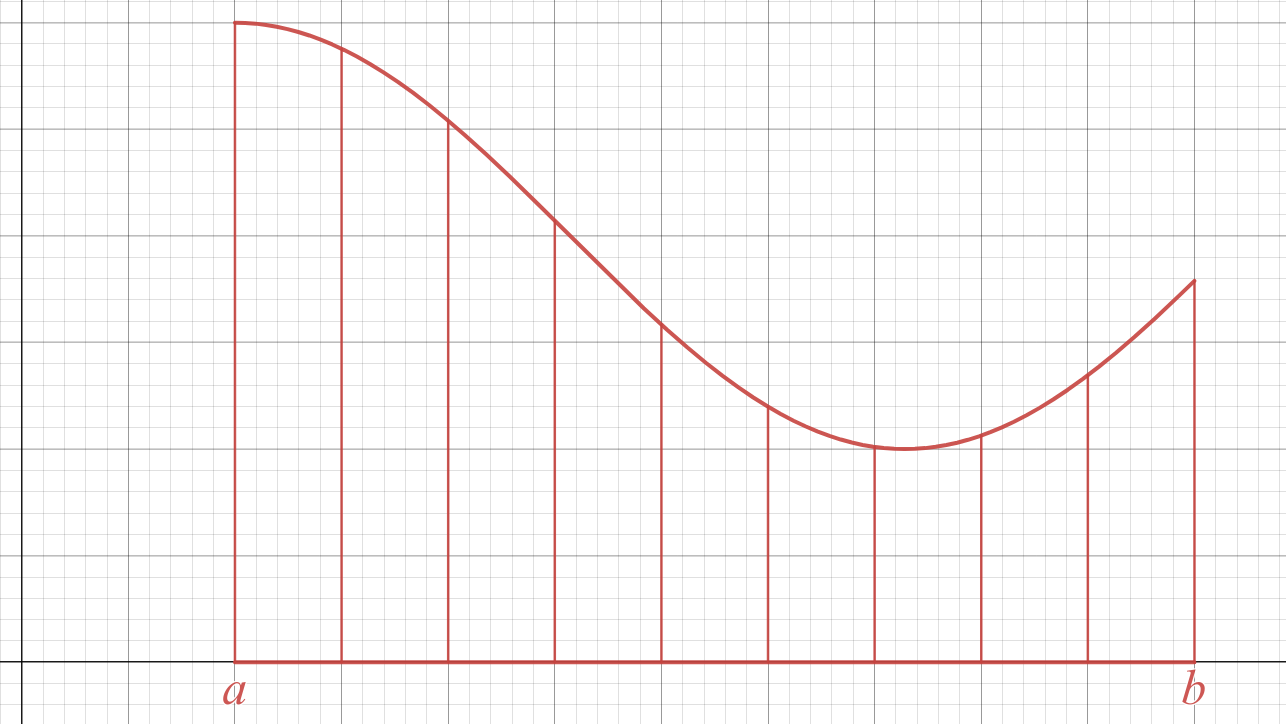
\includegraphics[scale=0.365]{regionSDivided}
		\end{center}
		\vspace*{10pt}
	\item Choose the left-end point for all subintervals: \\
	$x_0 = a$, $x_1 = a + \Delta x$, $\ldots$, $x_{n-2} = a + (n - 2) \Delta x$, $x_{n-1} = a + (n - 1) \Delta x$.
	\item Approximate by adding the area of each rectangle:
		\begin{align*}
		L_n = f(x_0) \Delta x + f(x_1) \Delta x + \cdots + f(x_{n-1}) \Delta x .
		\end{align*}
	\end{enumerate}
	
	\subsection{Sigma Notation}
	We use the symbol $\displaystyle \sum$ to write a summation of numbers compactly:
	
		\begin{center}
		\begin{tikzpicture}
		\draw (0,0)node[scale=3.0]{$\displaystyle\sum_{i=k}^n a_i$};
		\end{tikzpicture}
		\end{center}
	
	\begin{example}
	\begin{enumerate}[label=\textbf{\alph*)}]
	\item Expand $\displaystyle \sum_{i = 1}^7 i$.
	\item Write $\displaystyle 1 + \frac{1}{2} + \frac{1}{3} + \frac{1}{4} + \frac{1}{5} + \frac{1}{6} + \frac{1}{7}$ with the Sigma notation.
	\item Write $1 + 3 + 5 + 7 + 9 + 11 + 13$ with the Sigma notation.
	\end{enumerate}
	\end{example}
	
	\vfill
	
	\underline{Useful Sum Formulas:}
		
		\begin{itemize}
		\item $\displaystyle \sum_{i = 1}^n i = 1 + 2 + 3 + \cdots + n = \ \frac{n (n + 1)}{2}$;
		\item $\displaystyle  \sum_{i = 1}^n i^2 = 1^2 + 2^2 + \cdots + n^2 = \frac{n (n + 1) (2n + 1)}{6}$;
		\item $\displaystyle \sum_{i = 1}^n i^3 = 1^3 + 2^3 + \cdots + n^3 = \Big( \frac{n (n + 1)}{2} \Big)^2$.
		\end{itemize}
		
	\newpage
	
	\subsection{Taking the Limit!}
	
	\begin{example}
	Show that the area of the region $S$ in Example \ref{Ex:ParabolaArea} is $1/3$. In other words, show that
		\begin{align*}
		\mathrm{Area} (S) = \lim_{n \ra \infty} R_n = 1/3 .
		\end{align*}
	\end{example}
	
	\vfill
	
	\underline{General definition of Area:} The area of the region $S$ lying under the graph of a function $y = f(x)$ from $x = a$ to $x = b$ is given by
		\begin{itemize}
		\item $\mathrm{Area} (S) = \displaystyle\lim_{n \ra \infty} R_n =  \lim_{n \ra \infty} \Big( f(x_1) \Delta x + f(x_2) \Delta x + \cdots + f(x_n) \Delta x \Big)$ 
		\item $\mathrm{Area} (S) = \displaystyle\lim_{n \ra \infty} L_n = \lim_{n \ra \infty} \Big( f(x_0) \Delta x + f(x_1) \Delta x + \cdots + f(x_{n-1}) \Delta x \Big)$
		\end{itemize}
		
	\newpage
	
	\section{The Distance Problem}
	
	If an object move at constant velocity, then the distance between the start and finish line is easy to compute:
		\begin{center}
		\textsc{Distance} $=$ \textsc{Velocity} $\times$ $\Delta$\textsc{Time} .
		\end{center}
		
	What do we do if the velocity is not constant?
	
	\vspace*{12pt}
	
	\begin{example}
	Suppose the odometer on our car is broken and we want to estimate the distance driven over a $30$-second time interval. We take speedometer readings every five seconds and record them in the following table:
		\begin{center}
		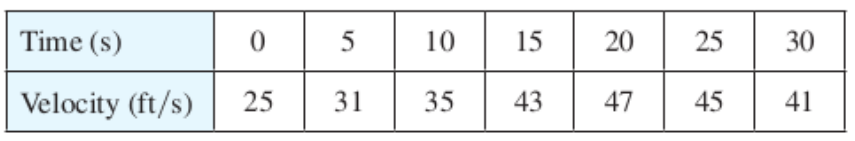
\includegraphics[scale=0.5]{tableVelocities.png}
		\end{center}
	\end{example}
	
	\vspace*{0.5cm}
	
	\begin{center}
	\begin{tikzpicture}
	\draw[black, very thick, ->, >=latex] (-0.5, 0) -- (14.5, 0);
	\draw[black, very thick, ->, >=latex] (0, -0.5) -- (0, 10.5);
	\foreach \i in { 10, 20, 30, 40, 50 } {
		\draw[black, thick] (0, {\i / 10 * 2}) -- (14.5, {\i / 10 * 2});
		\foreach \j in {1, 2, 3}{
			\draw[black!50] (0, {\i / 10 * 2 - \j * 0.5}) -- (14.5, {\i / 10 * 2 - \j * 0.5});}
		\draw[very thick] (-0.1, {\i / 10 * 2})node[left]{\i} -- (0.1, {\i / 10 * 2});}
	\foreach \i in { 5, 10, 15, 20, 25, 30, 35 } {
		\draw[black, thick] ({\i / 5 * 2}, 0) -- ({\i / 5 * 2}, 10.5);
		\foreach \j in {1, 2, 3} {
			\draw[black!50]({\i / 5 * 2 - \j * 0.5}, 0) -- ({\i / 5 * 2 - \j * 0.5}, 10.5);}
		\draw[very thick] ({\i / 5 * 2}, -0.1)node[below]{\i} -- ({\i / 5 * 2}, 0.1);}
	\end{tikzpicture}
	\end{center}
	
	\newpage
	
	\phantom{2}
	
	\vfill
	
	\underline{Remark:}
		\begin{itemize}
		\item The total distance is given by the area under the curve of the velocity function!
		\end{itemize}
	
\end{document}